\chapter{Sprint 3 : Suivi et Supervision}
\section{Introduction}
Fort des avancées réalisées dans les Sprints 1 et 2, qui ont mis en place les bases de l’accès, de l’administration et de la gestion des demandes, le Sprint 3 se focalise sur le suivi et la supervision au sein de la plateforme. Ce chapitre présente les fonctionnalités conçues pour permettre aux utilisateurs, managers, RH et administrateurs de superviser efficacement les processus, de consulter les demandes d’approbation, de suivre leurs équipes et de consulter les crédits de congés. Nous détaillerons les besoins identifiés, la conception de ces fonctionnalités et les étapes de leur mise en œuvre dans ce sprint.
\section{Backlog du Sprint 3}
Le tableau 5.1 représente le backlog du troisième sprint. Ce tableau détaille les cas d’utilisation, leurs priorités, estimations et tâches associées.
\begin{table}[!ht]
    \begin{adjustwidth}{-3.5cm}{-3.5cm}
        \vspace{-0.2cm}
    \centering
    \caption{Backlog du Sprint 3 : Suivi et Supervision}
    \label{tab:backlog_sprint3_suivi}
    \begin{tabular}{ | m{5cm} | m{1cm} | m{11.5cm} | }
    \hline
    \cellcolor[rgb]{0.832,0.832,0.832}Cas d'utilisation & \cellcolor[rgb]{0.832,0.832,0.832}Priorité & \cellcolor[rgb]{0.832,0.832,0.832}Tâche \\
    \hline
    Recevoir une notification & 2 & Utilisateurs, Managers et RH reçoivent des alertes sur des actions importantes. \\
    \hline
    Consulter les processus métiers & 3 & Administrateur consulte les processus métiers définis dans le système. \\
    \hline
    Consulter les demandes d’approbation & 3 & Administrateur accède aux demandes soumises pour consultation. \\
    \hline
    Consulter les membres de l’équipe & 3 & Utilisateurs, Managers et RH accèdent aux informations des membres de leur équipe. \\
    \hline
    Consulter ses crédits & 2 & Utilisateurs, Managers et RH vérifient leur solde de congés ou crédits. \\
    \hline
    \end{tabular}
    \end{adjustwidth}
\end{table}
\newpage
\section{Raffinement de cas d'utilisation} Cette partie consiste à analyser et spécifier les besoins de ce troisième sprint à travers l’identification des acteurs et le raffinement des cas d’utilisations.
\subsection{Identification des acteurs du troisième sprint} Les acteurs de ce sprint sont : \\
    \textbf{Utilisateur, Manager et RH} : Consulte les membres de son équipe, reçoit des notifications et consulte ses crédits. \\
    \textbf{Administrateur} : Consulte les processus métiers et les demandes d’approbation. \\
\subsection{Raffinement du cas d'utilisation <<Recevoir une notification>>}
La figure 5.1 illustre le diagramme de cas d’utilisation << Recevoir une notification >>
\begin{figure}[h]
    \centering
    \fbox{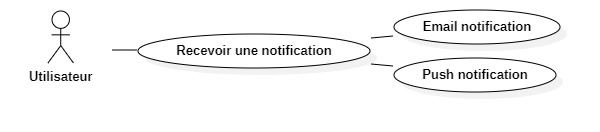
\includegraphics[width=11cm]{images/recnot.jpg}}
    \caption{Diagramme du cas d'utilisation <<Recevoir une notification>>}
    \label{fig:recnot}
\end{figure}\\
\begin{table}[!ht]
    \centering
    \caption{Description textuelle du Cas d’utilisation «Recevoir une notification par mail»}
    \label{tab:receive_email_notification}
    \renewcommand{\arraystretch}{1.2}
    \begin{tabular}{|p{4.2cm}|p{11cm}|}
    \hline
    \textbf{Cas d'utilisation} & Recevoir une notification par mail \\
    \hline
    \textbf{Acteur} & Utilisateur, Manager, RH \\
    \hline
    \textbf{Pré-conditions} & Système en marche. \newline Acteur authentifié. \newline Acteur a un e-mail valide configuré. \newline Une action importante a été déclenchée (ex. : demande traitée). \\
    \hline
    \textbf{Post-conditions} & L’acteur reçoit une notification par e-mail. \\
    \hline
    \textbf{Scénario de Base} & 
    1. Une action importante est effectuée (ex. : une demande est validée ou rejetée). \newline
    2. Le système génère une notification avec les détails de l’action. \newline
    3. Le système envoie un e-mail à l’adresse de l’acteur concerné. \newline
    4. L’acteur consulte l’e-mail dans sa boîte de réception. \\
    \hline
    \textbf{Exceptions} & 
    Échec d’envoi (e-mail invalide, problème de serveur SMTP, erreur API). \\
    \hline
    \end{tabular}
    \end{table}
    \newpage
    \begin{table}[!ht]
        \centering
        \caption{Description textuelle du Cas d’utilisation «Recevoir une notification push»}
        \label{tab:receive_push_notification_websocket}
        \renewcommand{\arraystretch}{1.2}
        \begin{tabular}{|p{4.2cm}|p{11cm}|}
        \hline
        \textbf{Cas d'utilisation} & Recevoir une notification push \\
        \hline
        \textbf{Acteur} & Utilisateur, Manager, RH \\
        \hline
        \textbf{Pré-conditions} & Système en marche. \newline Manager authentifié. \newline Manager connecté à l’application avec une session WebSocket active. \newline Une demande est soumise ou traitée (ex. : validation/rejet par RH). \\
        \hline
        \textbf{Post-conditions} & Le manager reçoit une notification push en temps réel. \\
        \hline
        \textbf{Scénario de Base} & 
        1. Une demande est soumise par un utilisateur ou traitée par un autre acteur (ex. : RH). \newline
        2. Le système génère une notification avec les détails (ex. : type de demande, statut). \newline
        3. Le serveur Spring WebSocket envoie la notification au client du manager via la connexion WebSocket. \newline
        4. La notification s’affiche en temps réel dans l’interface du manager (ex. : pop-up ou badge). \\
        \hline
        \textbf{Exceptions} & 
        Échec de réception (connexion WebSocket interrompue, manager hors ligne, erreur serveur). \\
        \hline
        \end{tabular}
        \end{table}
\subsection{Raffinement du cas d'utilisation <<Consulter les processus métiers>>}
La figure~\ref{fig:cpmet} illustre le diagramme de cas d'utilisation « Consulter les processus métiers ».
\begin{figure}[h]
     \centering
     \fbox{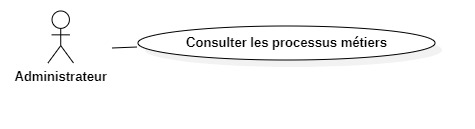
\includegraphics[width=13cm]{images/cpm.jpg}}
     \caption{Diagramme du cas d'utilisation <<Consulter les processus métiers>>}
     \label{fig:cpmet}
\end{figure}\\
\newpage
\begin{table}[!ht]
    \begin{adjustwidth}{-2cm}{-2cm}
    \centering
    \caption{Description textuelle du Cas d'utilisation «Consulter les processus métiers»}
    \label{tab:consult_business_processes}
    \renewcommand{\arraystretch}{1.2}
    \begin{tabular}{|p{4.2cm}|p{13cm}|}
    \hline
    \textbf{Cas d'utilisation} & Consulter les processus métiers \\
    \hline
    \textbf{Acteur} & Administrateur \\
    \hline
    \textbf{Pré-conditions} & 
    \begin{itemize}
    \item Système en marche
    \item Administrateur authentifié
    \item Processus métiers déjà définis dans le système
    \end{itemize} \\
    \hline
    \textbf{Post-conditions} & L'administrateur visualise la liste des processus métiers configurés. \\
    \hline
    \textbf{Scénario de Base} & 
    \begin{enumerate}
    \item L'administrateur accède à la section "Processus métiers"
    \item Le système récupère et affiche la liste des processus
    \item L'administrateur peut visualiser un processus spécifique
    \item Le système affiche les modèle BPMN du processus sélectionné
    \end{enumerate} \\
    \hline
    \textbf{Exceptions} & 
    \begin{itemize}
    \item Aucun processus défini → Message "Aucun processus disponible"
    \item Erreur de chargement → Notification d'erreur technique
    \end{itemize} \\
    \hline
    \end{tabular}
    \end{adjustwidth}
    \end{table}
\subsection{Raffinement du cas d'utilisation <<Consulter les demandes d'approbation>>}
La figure~\ref{fig:cpmet} illustre le diagramme de cas d'utilisation « Consulter les demandes d'approbation ».
\begin{figure}[h]
     \centering
     \fbox{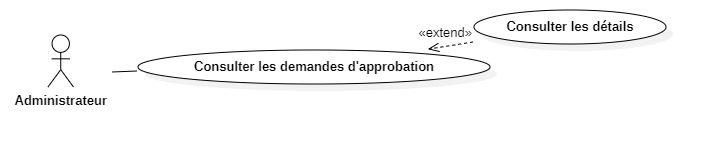
\includegraphics[width=13cm]{images/cdapp.jpg}}
     \caption{Diagramme du cas d'utilisation <<Consulter les demandes d'approbation>>}
     \label{fig:cdapp}
\end{figure}\\
\newpage
\begin{table}[!ht]
    \vspace{-1.5cm}
    \begin{adjustwidth}{-2cm}{-2cm}
    \centering
    \caption{Description textuelle du Cas d'utilisation «Consulter les demandes d'approbation»}
    \label{tab:cdapp}
    \renewcommand{\arraystretch}{1.2}
    \begin{tabular}{|p{4.2cm}|p{13cm}|}
    \hline
    \textbf{Cas d'utilisation} & Consulter les demandes d'approbation \\
    \hline
    \textbf{Acteur} & Administrateur \\
    \hline
    \textbf{Pré-conditions} & 
    \begin{itemize}
    \item Système en marche
    \item Administrateur authentifié
    \item Demandes soumises par les utilisateurs
    \end{itemize} \\
    \hline
    \textbf{Post-conditions} & L'administrateur visualise les demandes en attente ou historiques. \\
    \hline
    \textbf{Scénario de Base} & 
    \begin{enumerate}
    \item L'administrateur accède à la section "Demandes d'approbation"
    \item Le système récupère les demandes (filtrables par statut/date/type)
    \item L'administrateur sélectionne une demande pour en voir les détails
    \item Optionnel : Export des données en PDF
    \end{enumerate} \\
    \hline
    \textbf{Exceptions} & 
    \begin{itemize}
    \item Aucune demande disponible → Afficher "Aucune demande trouvée"
    \item Données corrompues → Proposer une réinitialisation du filtre
    \end{itemize} \\
    \hline
    \end{tabular}
    \end{adjustwidth}
    \end{table}
    \begin{table}[!ht]
        \begin{adjustwidth}{-2cm}{-2cm}
        \centering
        \caption{Description textuelle du Cas d'utilisation «Consulter les détails d'une demande d'approbation»}
        \label{tab:consult_request_details}
        \renewcommand{\arraystretch}{1.2}
        \begin{tabular}{|p{4.2cm}|p{13cm}|}
        \hline
        \textbf{Cas d'utilisation} & Consulter les détails d'une demande d'approbation \\
        \hline
        \textbf{Acteur} & Administrateur\\
        \hline
        \textbf{Pré-conditions} & 
        \begin{itemize}
        \item Système en marche
        \item Utilisateur authentifié et autorisé
        \item Demande existante dans le système
        \end{itemize} \\
        \hline
        \textbf{Post-conditions} & L'utilisateur visualise tous les détails de la demande sélectionnée. \\
        \hline
        \textbf{Scénario de Base} & 
        \begin{enumerate}
        \item L'utilisateur sélectionne une demande dans la liste
        \item Le système affiche les informations principales
        \item L'utilisateur clique sur "Voir détails complets
        \item Le système affiche les détails de la demande
        \end{enumerate} \\
        \hline
        \textbf{Extensions} & 
        \begin{itemize}
        \item Impression des avis de congé : génération d'un PDF
        \end{itemize} \\
        \hline
        \textbf{Exceptions} & 
        \begin{itemize}
        \item Accès non autorisé → Redirection vers page d'erreur
        \item Pièces jointes corrompues → Notification spécifique
        \end{itemize} \\
        \hline
        \end{tabular}
        \end{adjustwidth}
        \end{table}
\newpage
\subsection{Raffinement du cas d'utilisation <<Consulter les membres de l'équipe>>}
La figure~\ref{fig:cmequipe} illustre le diagramme de cas d'utilisation « Consulter les membres de l'équipe ».
\begin{figure}[h]
     \centering
     \fbox{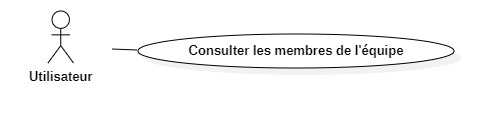
\includegraphics[width=11cm]{images/cmequipe.jpg}}
     \caption{Diagramme du cas d'utilisation <<Consulter les membres de l'équipe>>}
     \label{fig:cmequipe}
\end{figure}
\begin{table}[!ht]
    \begin{adjustwidth}{-2cm}{-2cm}
    \centering
    \caption{Description textuelle du Cas d'utilisation «Consulter les membres de l'équipe»}
    \label{tab:consult_team_members}
    \renewcommand{\arraystretch}{1.2}
    \begin{tabular}{|p{4.2cm}|p{11cm}|}
    \hline
    \textbf{Cas d'utilisation} & Consulter les membres de l'équipe \\
    \hline
    \textbf{Acteurs} & Utilisateurs, Managers, RH \\
    \hline
    \textbf{Pré-conditions} & 
    \begin{itemize}
    \item Système en marche
    \item Utilisateur authentifié
    \end{itemize} \\
    \hline
    \textbf{Post-conditions} & Visualisation des profils des membres de l'équipe. \\
    \hline
    \textbf{Scénario de Base} & 
    \begin{enumerate}
    \item L'utilisateur accède à la section "Équipe"
    \item Le système affiche la liste des membres
    \item L'utilisateur clique sur un membre pour voir plus de détails
    \item Optionnel : Recherche par nom/fonction
    \end{enumerate} \\
    \hline
    \textbf{Exceptions} & 
    \begin{itemize}
    \item Équipe vide → Afficher "Aucun membre trouvé"
    \item Accès refusé → Rediriger vers une page d'erreur 403
    \end{itemize} \\
    \hline
    \end{tabular}
    \end{adjustwidth}
    \end{table}
    \subsection{Raffinement du cas d'utilisation <<Consulter ses crédits>>}
La figure~\ref{fig:cscredits} illustre le diagramme de cas d'utilisation « Consulter ses crédits ».
\newpage
\begin{figure}[h]
     \centering
     \fbox{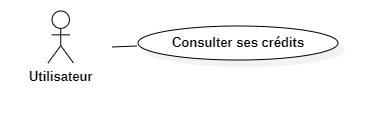
\includegraphics[width=11cm]{images/cscredits.jpg}}
     \caption{Diagramme du cas d'utilisation <<Consulter ses crédits>>}
     \label{fig:cscredits}
\end{figure}
\begin{table}[!ht]
    \begin{adjustwidth}{-2cm}{-2cm}
    \centering
    \caption{Description textuelle du Cas d'utilisation «Consulter ses crédits»}
    \label{tab:consult_credits}
    \renewcommand{\arraystretch}{1.2}
    \begin{tabular}{|p{4.2cm}|p{11cm}|}
    \hline
    \textbf{Cas d'utilisation} & Consulter ses crédits \\
    \hline
    \textbf{Acteurs} & Utilisateurs, Managers, RH \\
    \hline
    \textbf{Pré-conditions} & 
    \begin{itemize}
    \item Système en marche
    \item Utilisateur authentifié
    \item Crédits/congés déjà attribués
    \end{itemize} \\
    \hline
    \textbf{Post-conditions} & Visualisation du solde de crédits(congés,autorisations) disponibles. \\
    \hline
    \textbf{Scénario de Base} & 
    \begin{enumerate}
    \item L'utilisateur accède à la section "Menu principal"
    \item Le système affiche le solde disponible
    \end{enumerate} \\
    \hline
    \textbf{Exceptions} & 
    \begin{itemize}
    \item Données non chargées → Afficher "Données non chargées"
    \item Crédits non attribués → Afficher "Solde non disponible"
    \end{itemize} \\
    \hline
    \end{tabular}
    \end{adjustwidth}
\end{table}

\section{Conception}
Dans cette partie nous allons exposer la conception des cas d’utilisations de ce sprint qui se traduit par un diagramme de 
classe globale de ce sprint suivi par les diagrammes de classes et les diagrammes de séquences de chaque cas d’utilisation.
La figure~\ref{fig:class_diagram_sprint3} illustre le diagramme de classe du Sprint 2.\\
\newpage
\subsection{Diagramme de classe du sprint 3}
\begin{figure}[h]
     \centering
     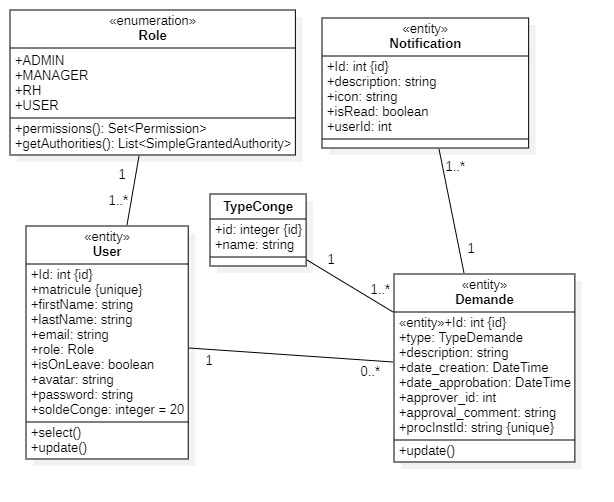
\includegraphics[width=15cm]{images/csprint3.jpg}
     \caption{Diagramme de classe du Sprint 3}
     \label{fig:class_diagram_sprint3}
\end{figure}
Le diagramme présente l'architecture objet centrale avec :\\
\begin{itemize}
    \item \textbf{Énumération "Role"} : Définit les rôles système.
    \item \textbf{Classe "User"} : Modélise les utilisateurs.
    \item \textbf{Classe "TypeConge"} : Structure les types de congés disponibles.
    \item \textbf{Classe "Notification"} : Gère le système d'alertes.
    \item \textbf{Classe "Demande"} : Traite les requêtes utilisateurs.
\end{itemize}
\newpage
\vspace{-1cm}
\subsection{Conception du cas d’utilisation «Recevoir une notification»}
\subsubsection{Diagramme de Classe}
La figure~\ref{fig:class_notif_rec} illustre le diagramme de classes du cas d'utilisation « Recevoir une notification ».
\begin{figure}[h]
     \centering
     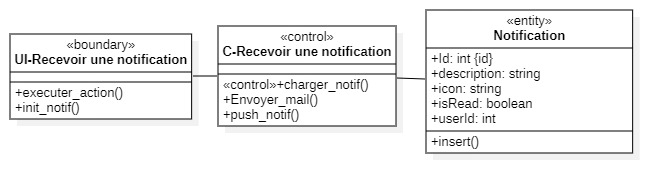
\includegraphics[width=14cm]{images/C_recnot.jpg}
     \caption{Diagramme de classe du cas d'utilisation <<Recevoir une notification>>}
     \label{fig:class_notif_rec}
\end{figure}
\subsubsection{Diagramme de Séquence}
L'utilisateur déclenche une action qui initialise une notification via le contrôleur. Le contrôleur charge les données, envoie un email si l'action nécessite une notification par email. Sinon, il insère une notification push.
Ce scénario est modélisé dans la figure \ref{fig:S_notif_rec}.
\begin{figure}[ht]
    \centering
    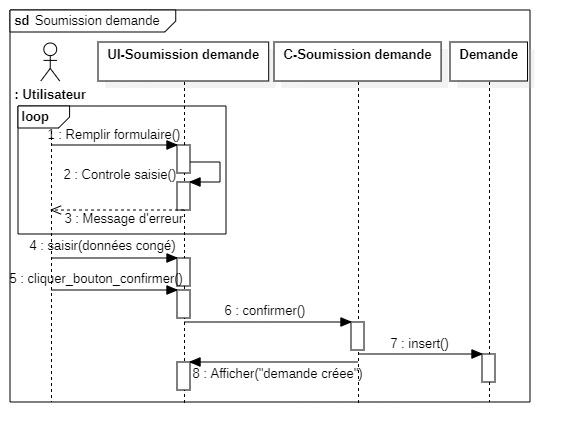
\includegraphics[width=13cm, height=0.9\textheight, keepaspectratio]{images/S_Soumission demande.jpg}
    \caption{Diagramme de séquence du cas d'utilisation <<Recevoir une notification>>}
    \label{fig:S_notif_rec}
\end{figure}
\newpage
\subsection{Conception du cas d’utilisation «Consulter les processus métiers»}
\subsubsection{Diagramme de Classe}
La figure~\ref{fig:c_cpmet} illustre le diagramme de classes du cas d'utilisation « Consulter les processus métiers ».
\begin{figure}[h]
     \centering
     \includegraphics[width=14cm]{images/c_cpmet.jpg}
     \caption{Diagramme de classe du cas d'utilisation <<Consulter les processus métiers>>}
     \label{fig:c_cpmet}
\end{figure}
\subsubsection{Diagramme de Séquence}
L'administrateur se connecte, clique sur "Processus métiers" dans le menu principal, sélectionne un processus dans la liste affichée, et consulte le diagramme BPMN interactif avec ses étapes et règles associées.Ce scénario est modélisé dans la figure \ref{fig:S_cpmet}.
\begin{figure}[ht]
    \centering
    \includegraphics[width=13cm, height=0.9\textheight, keepaspectratio]{images/s_cpmet.jpg}
    \caption{Diagramme de séquence du cas d'utilisation <<Consulter les processus métiers>>}
    \label{fig:S_cpmet}
\end{figure}
\newpage
\vspace*{-2cm}
\subsection{Conception du cas d’utilisation «Consulter les demandes d’approbation»}
\subsubsection{Diagramme de Classe}
La figure~\ref{fig:c_cdapprob} illustre le diagramme de classes du cas d'utilisation « Consulter les demandes d’approbation ».
\begin{figure}[h]
     \centering
     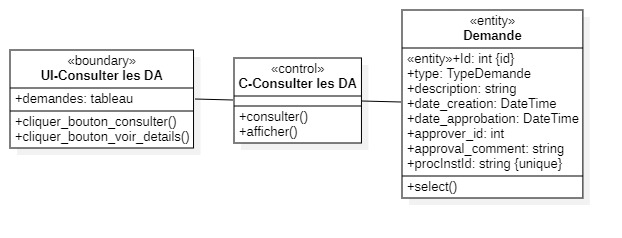
\includegraphics[width=13cm]{images/c_cdapprob.jpg}
     \caption{Diagramme de classe du cas d'utilisation <<Consulter les demandes d’approbation>>}
     \label{fig:c_cdapprob}
\end{figure}
\subsubsection{Diagramme de Séquence}
L'administrateur consulte la liste des demandes, clique sur une demande pour afficher les détails complets (historique, documents joints, commentaires).
\begin{figure}[ht]
    \centering
    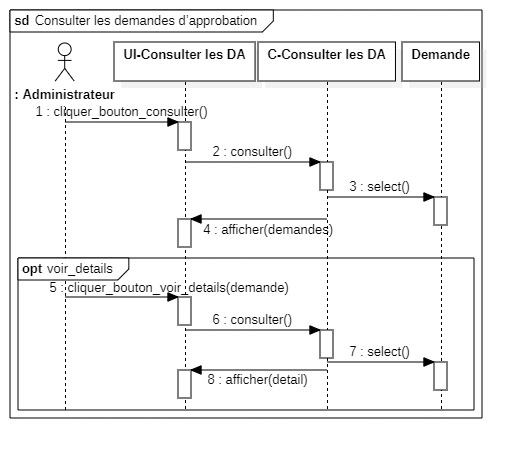
\includegraphics[width=11cm, height=0.8\textheight, keepaspectratio]{images/s_cdapprob.jpg}
    \caption{Diagramme de séquence du cas d'utilisation <<Consulter les demandes d’approbation>>}
    \label{fig:s_cdapprob}
\end{figure}
\newpage
\vspace*{-1.5cm}
\subsection{Conception du cas d’utilisation «Consulter les membres de l’équipe»}
\subsubsection{Diagramme de Classe}
La figure~\ref{fig:c_cmemeq} illustre le diagramme de classes du cas d'utilisation « Consulter les membres de l’équipe ».
\begin{figure}[h]
     \centering
     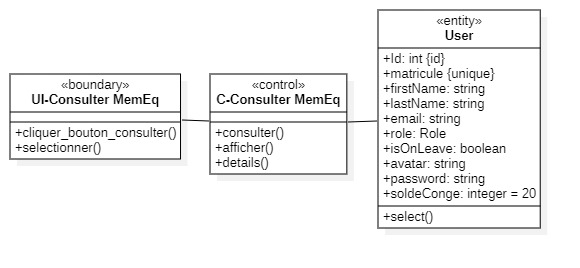
\includegraphics[width=13cm]{images/c_cmemeq.jpg}
     \caption{Diagramme de classe du cas d'utilisation <<Consulter les membres de l’équipe>>}
     \label{fig:c_cmemeq}
\end{figure}
\subsubsection{Diagramme de Séquence}
L'utilisateur consulte la liste des membres de son équipe, clique sur un collaborateur pour afficher ses détails (email).
\begin{figure}[ht]
    \centering
    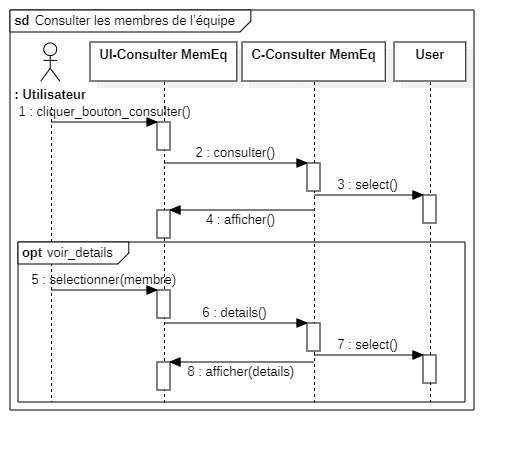
\includegraphics[width=10cm, height=0.8\textheight, keepaspectratio]{images/s_cmemeq.jpg}
    \caption{Diagramme de séquence du cas d'utilisation <<Consulter les membres de l’équipe>>}
    \label{fig:S_cmemeq}
\end{figure}
\subsection{Conception du cas d’utilisation «Consulter ses crédits»}
\subsubsection{Diagramme de Classe}
La figure~\ref{fig:c_cscred} illustre le diagramme de classes du cas d'utilisation « Consulter ses crédits ».
\begin{figure}[h]
     \centering
     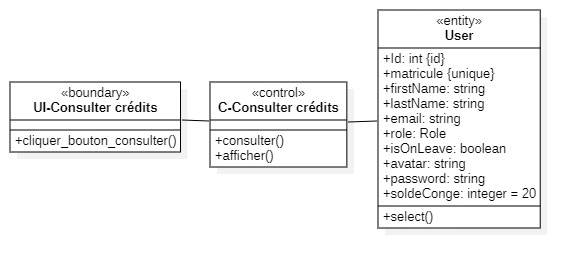
\includegraphics[width=14cm]{images/c_cscred.jpg}
     \caption{Diagramme de classe du cas d'utilisation <<Consulter ses crédits>>}
     \label{fig:c_cscred}
\end{figure}\\
L'utilisateur clique sur le bouton du menu principal, il consulte son solde de crédits disponibles (congés, autorisation) dans son espace personnel.
\begin{figure}[ht]
    \centering
    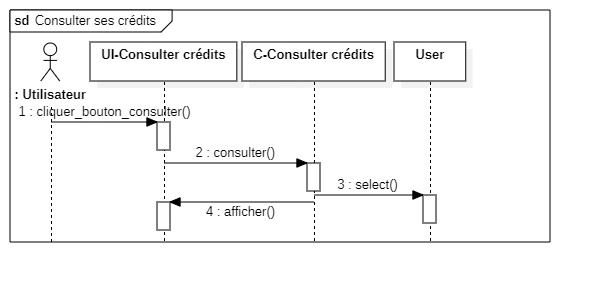
\includegraphics[width=13cm, height=0.8\textheight, keepaspectratio]{images/s_cscred.jpg}
    \caption{Diagramme de séquence du cas d'utilisation <<Consulter ses crédits>>}
    \label{fig:S_cscred}
\end{figure}
\newpage
\section{Réalisation}
Dans cette partie, nous présentons les modules de notre troisième sprint en utilisant des captures d’écran.
\subsection{Recevoir une notification}
La figure~\ref{fig:notifications} présente le centre de notifications unifié.
\begin{figure}[h]
    \centering
    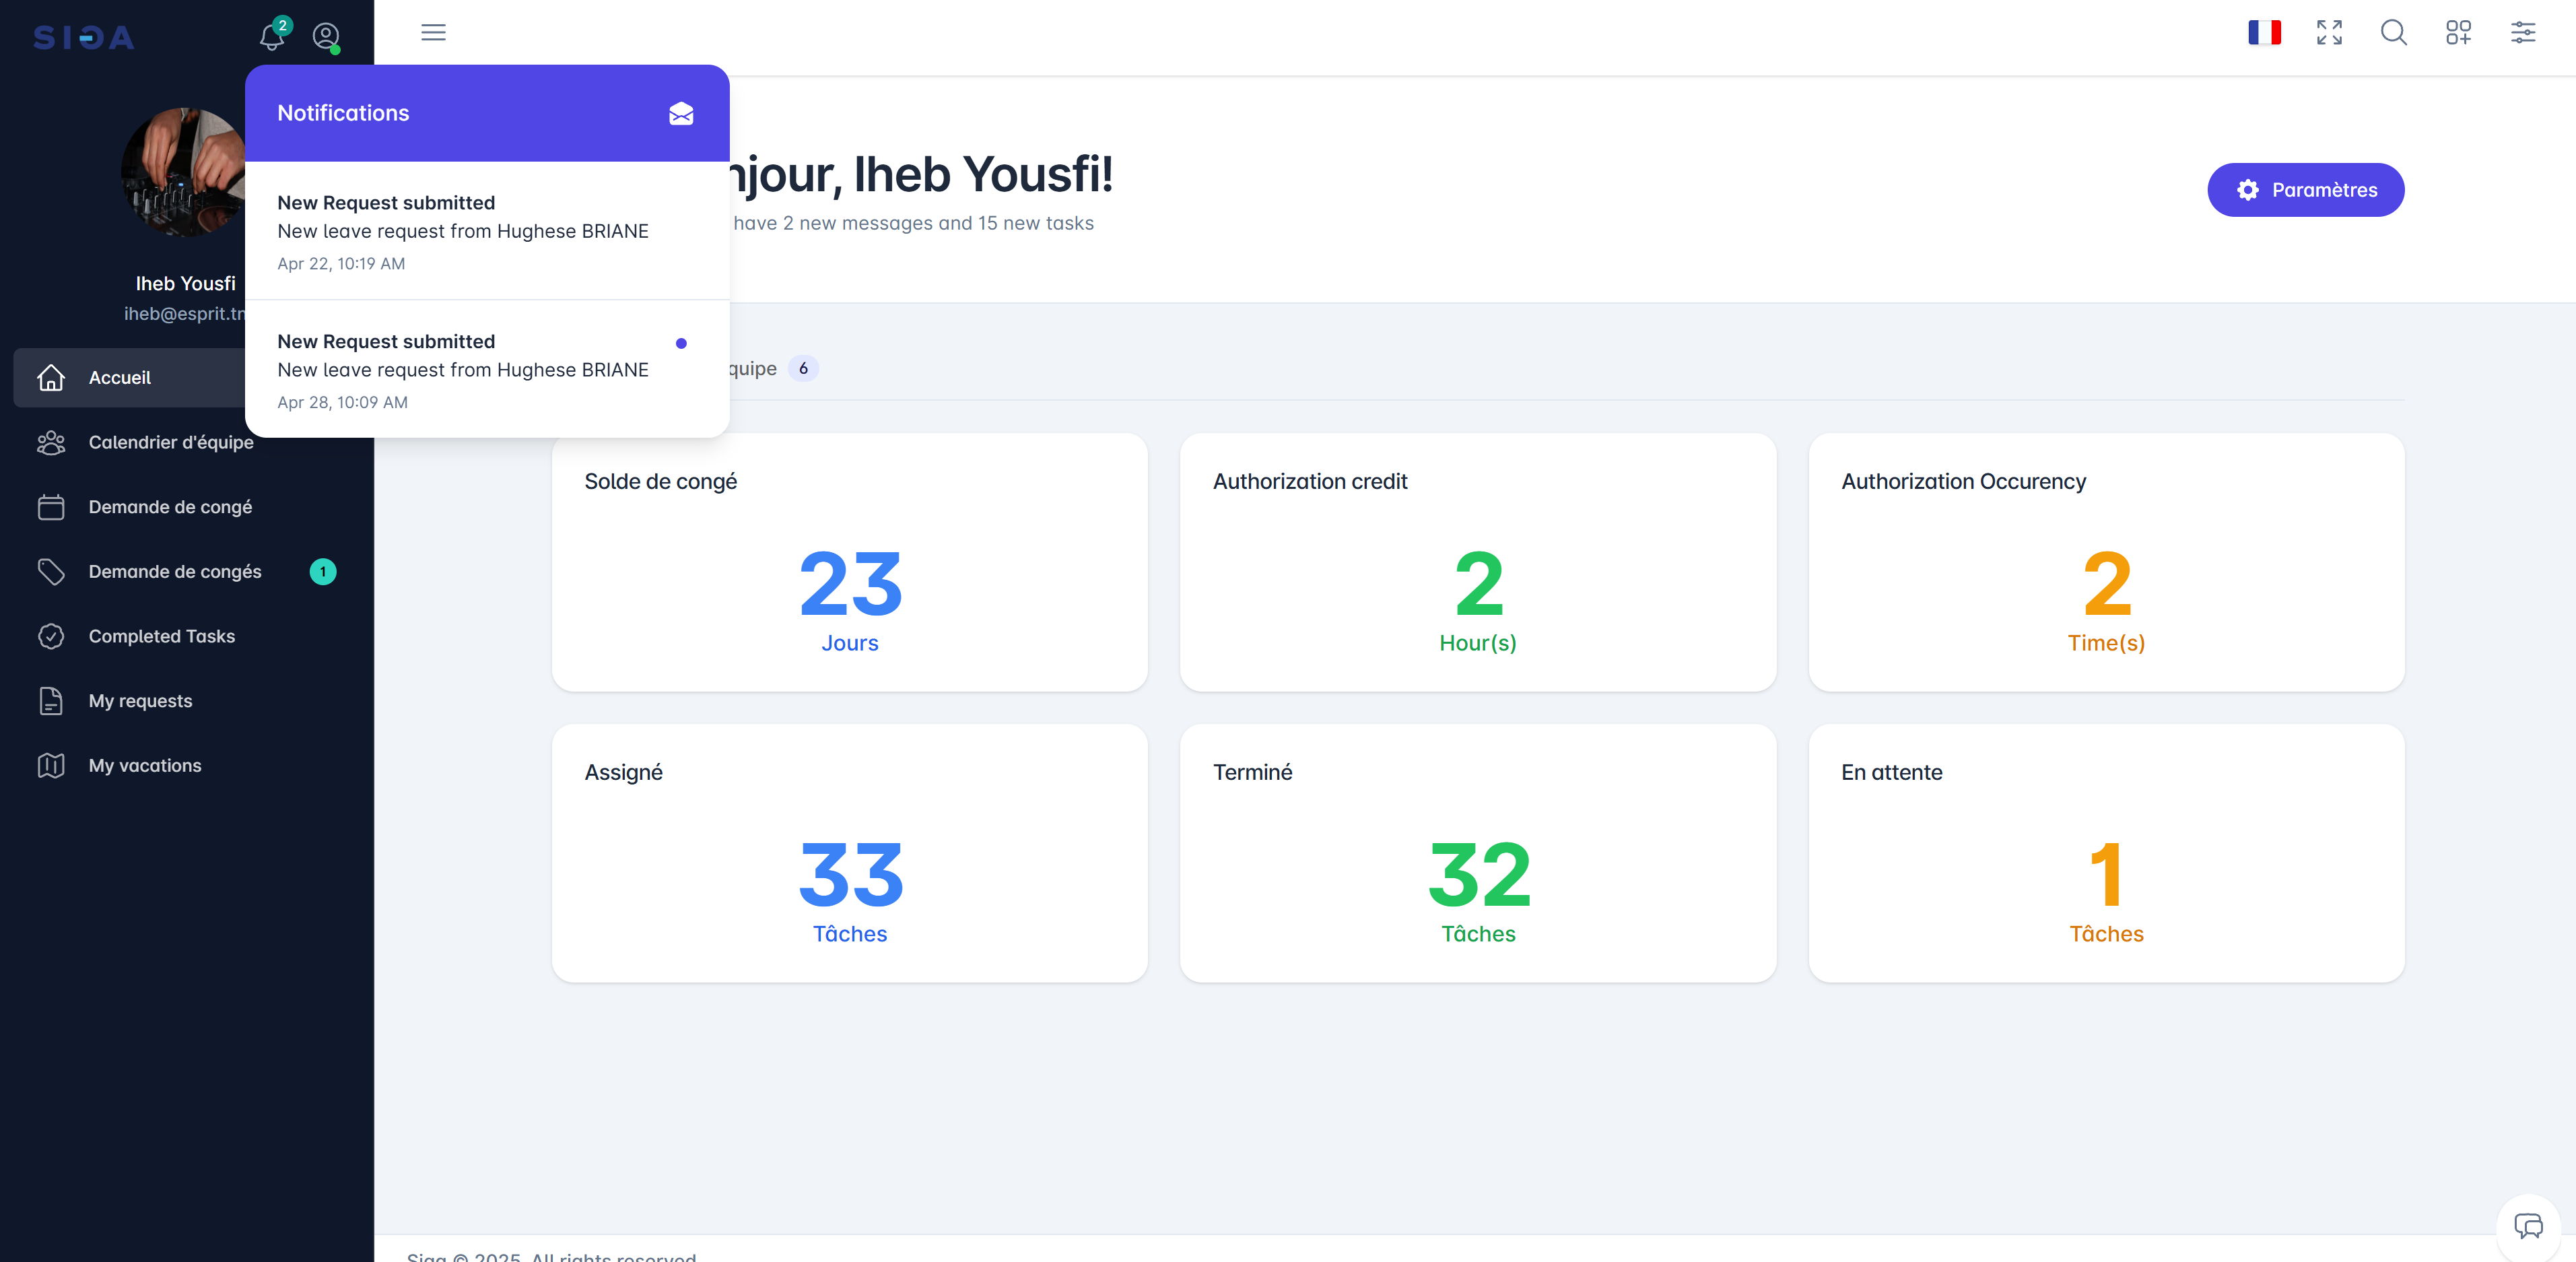
\includegraphics[width=16cm]{images/realisation/notif.png}
    \caption{Interface du cas d'utilisation «Recevoir une notification»}
    \label{fig:notifications}
\end{figure}

\subsection{Consulter les processus métiers}
La figure~\ref{fig:processus} présente l'interface permettant aux administrateurs de consulter les workflows métiers.
\newpage
\begin{figure}[h]
    \centering
    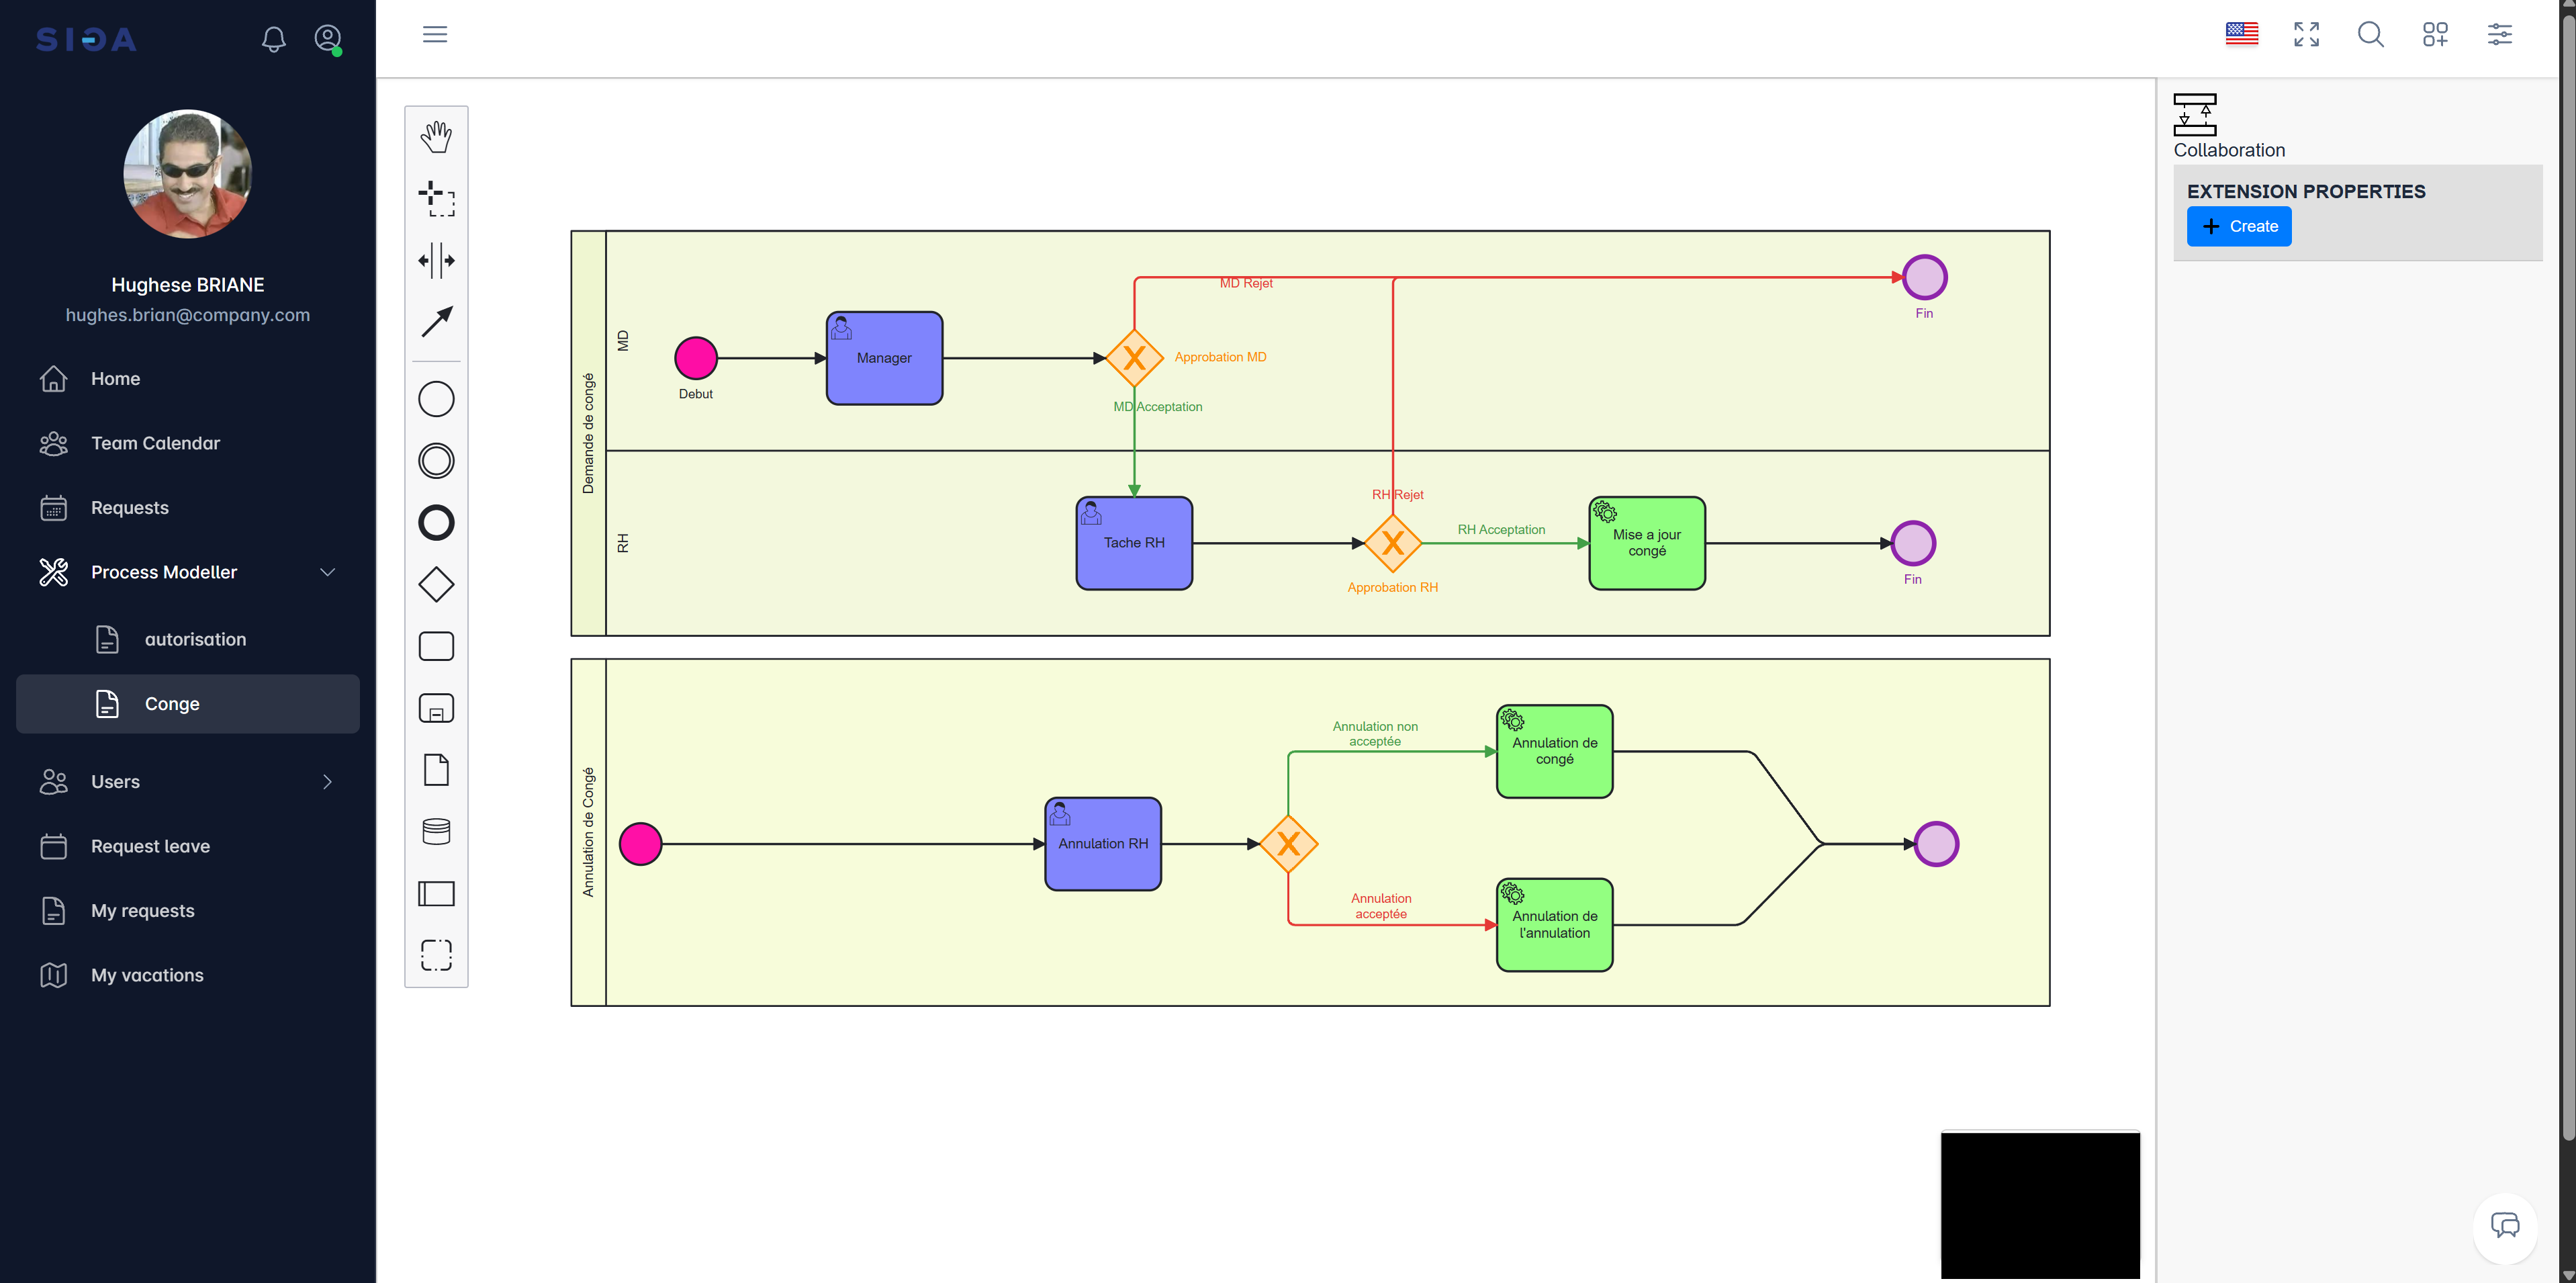
\includegraphics[width=16cm]{images/realisation/processes.png}
    \caption{Interface du cas d'utilisation «Consulter les processus métiers»}
    \label{fig:processus}
\end{figure}
\subsection{Consulter les demandes d’approbation}
Les figure~\ref{fig:demandes} et \ref{fig:demandes2} illustrent l'interface de consultation des demandes avec :
\begin{itemize}
    \item Les détails de chaque demande
    \item L'historique complet des décisions
    \item Filtrage multi-critères
    \item Recherche dynamique sur toutes les colonnes
\end{itemize}

\begin{figure}[h]
    \centering
    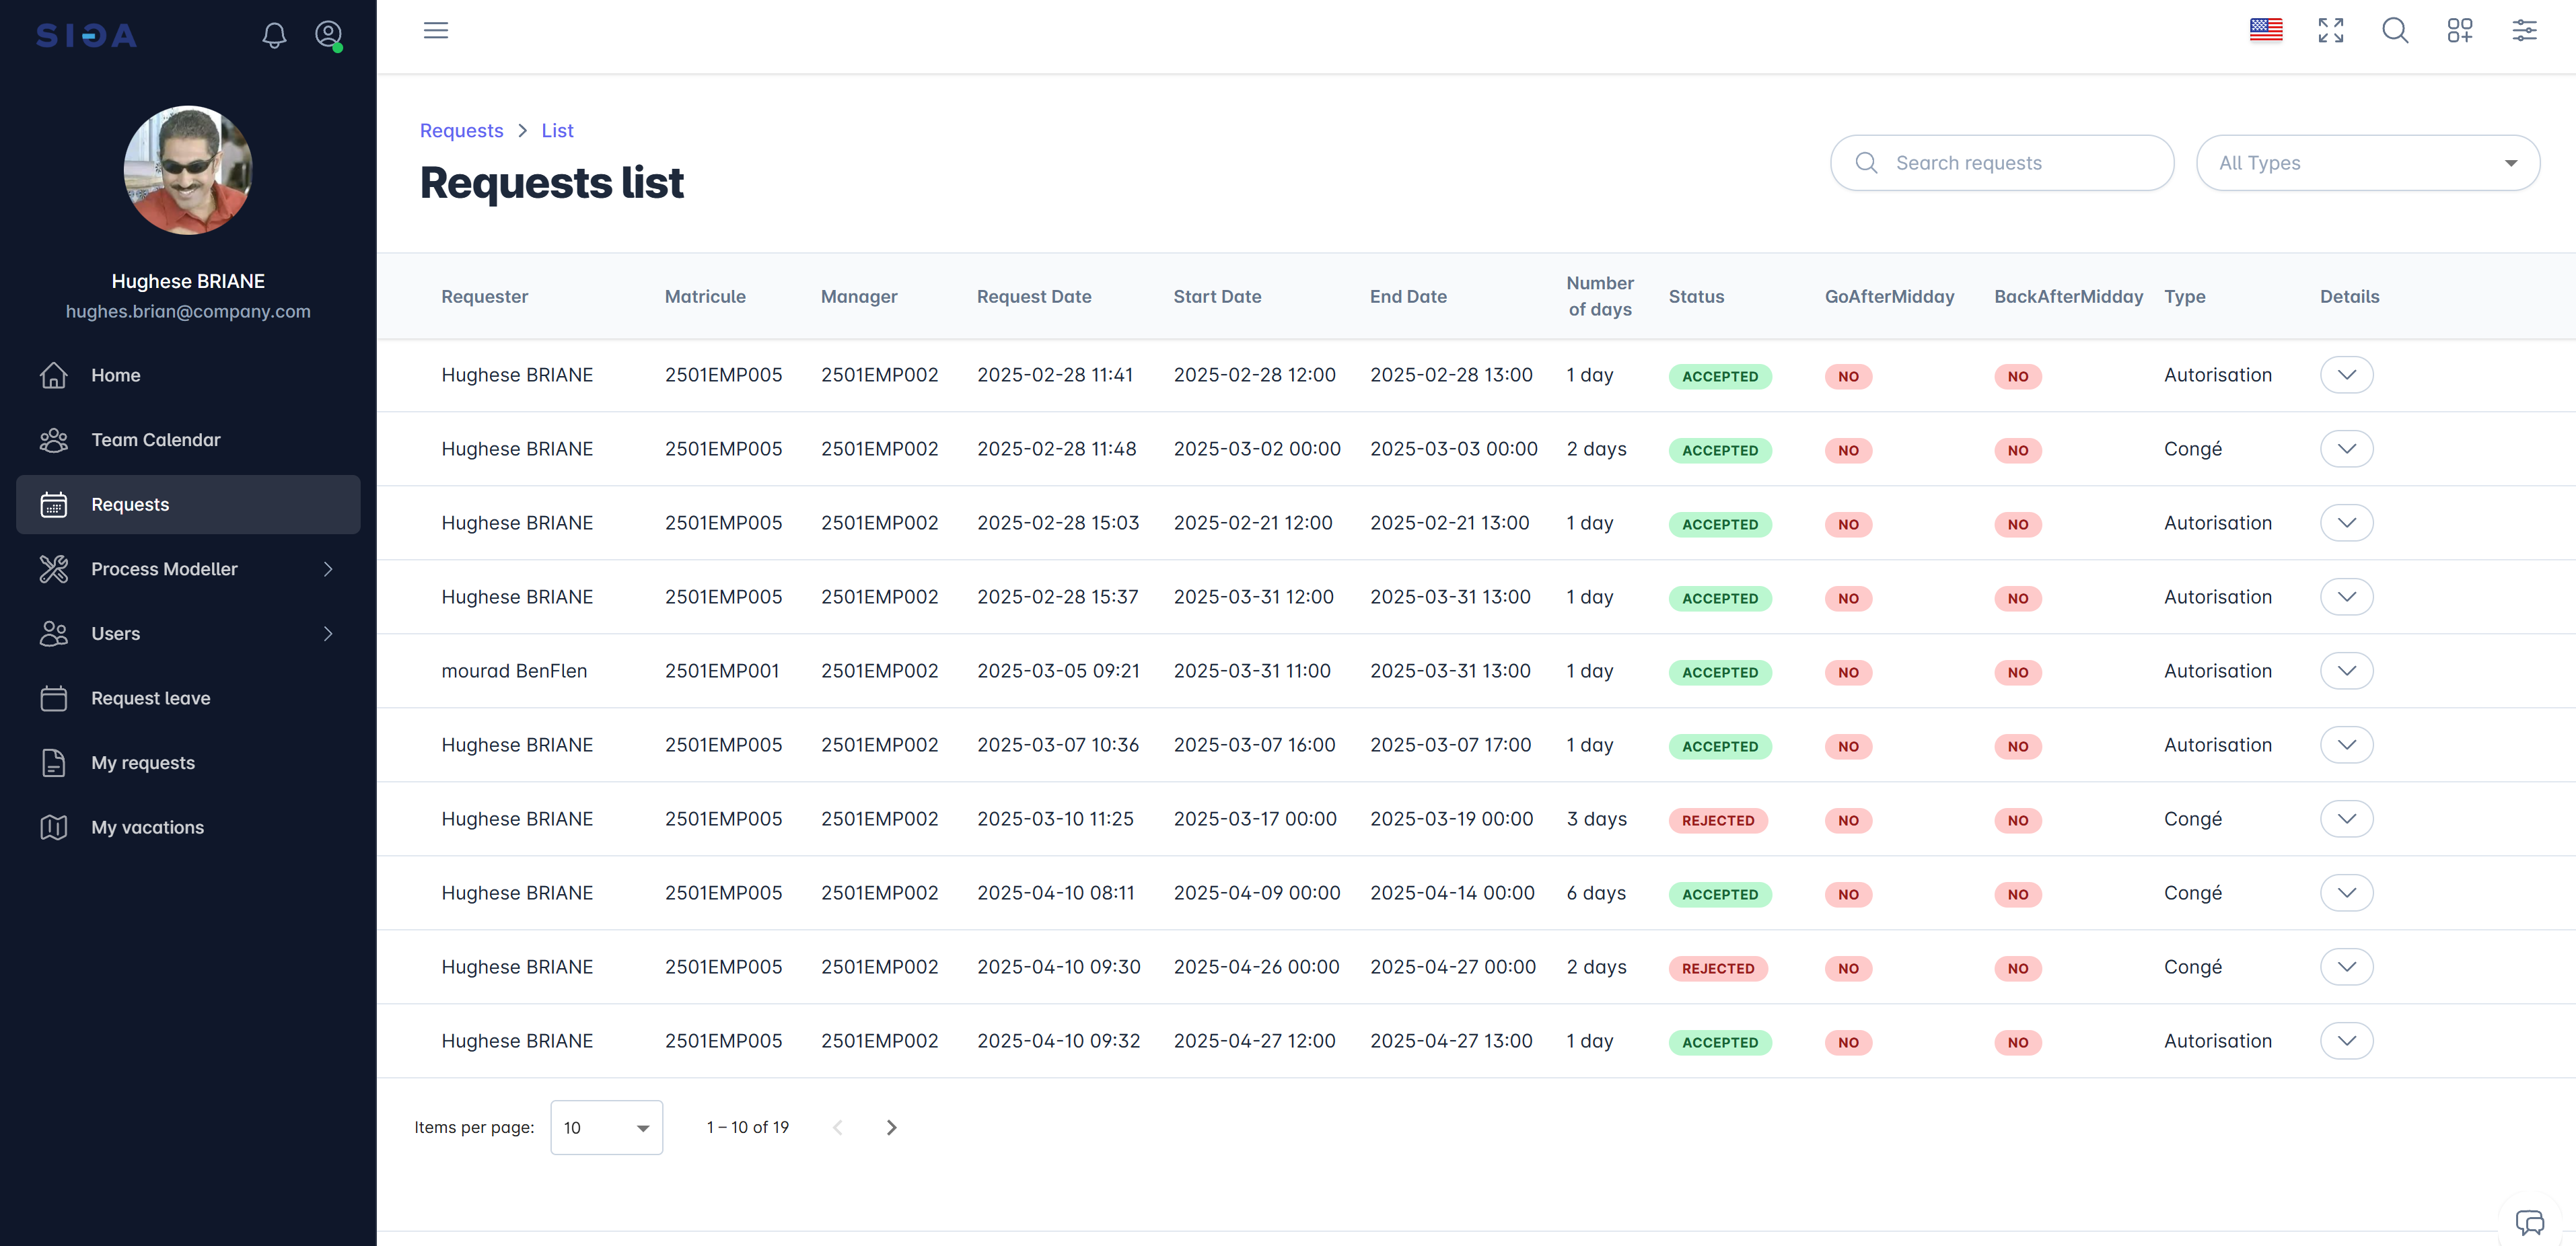
\includegraphics[width=16cm]{images/realisation/req1.png}
    \caption{Interface du cas d'utilisation «Consulter les demandes d’approbation»}
    \label{fig:demandes}
\end{figure}
\begin{figure}[h]
    \centering
    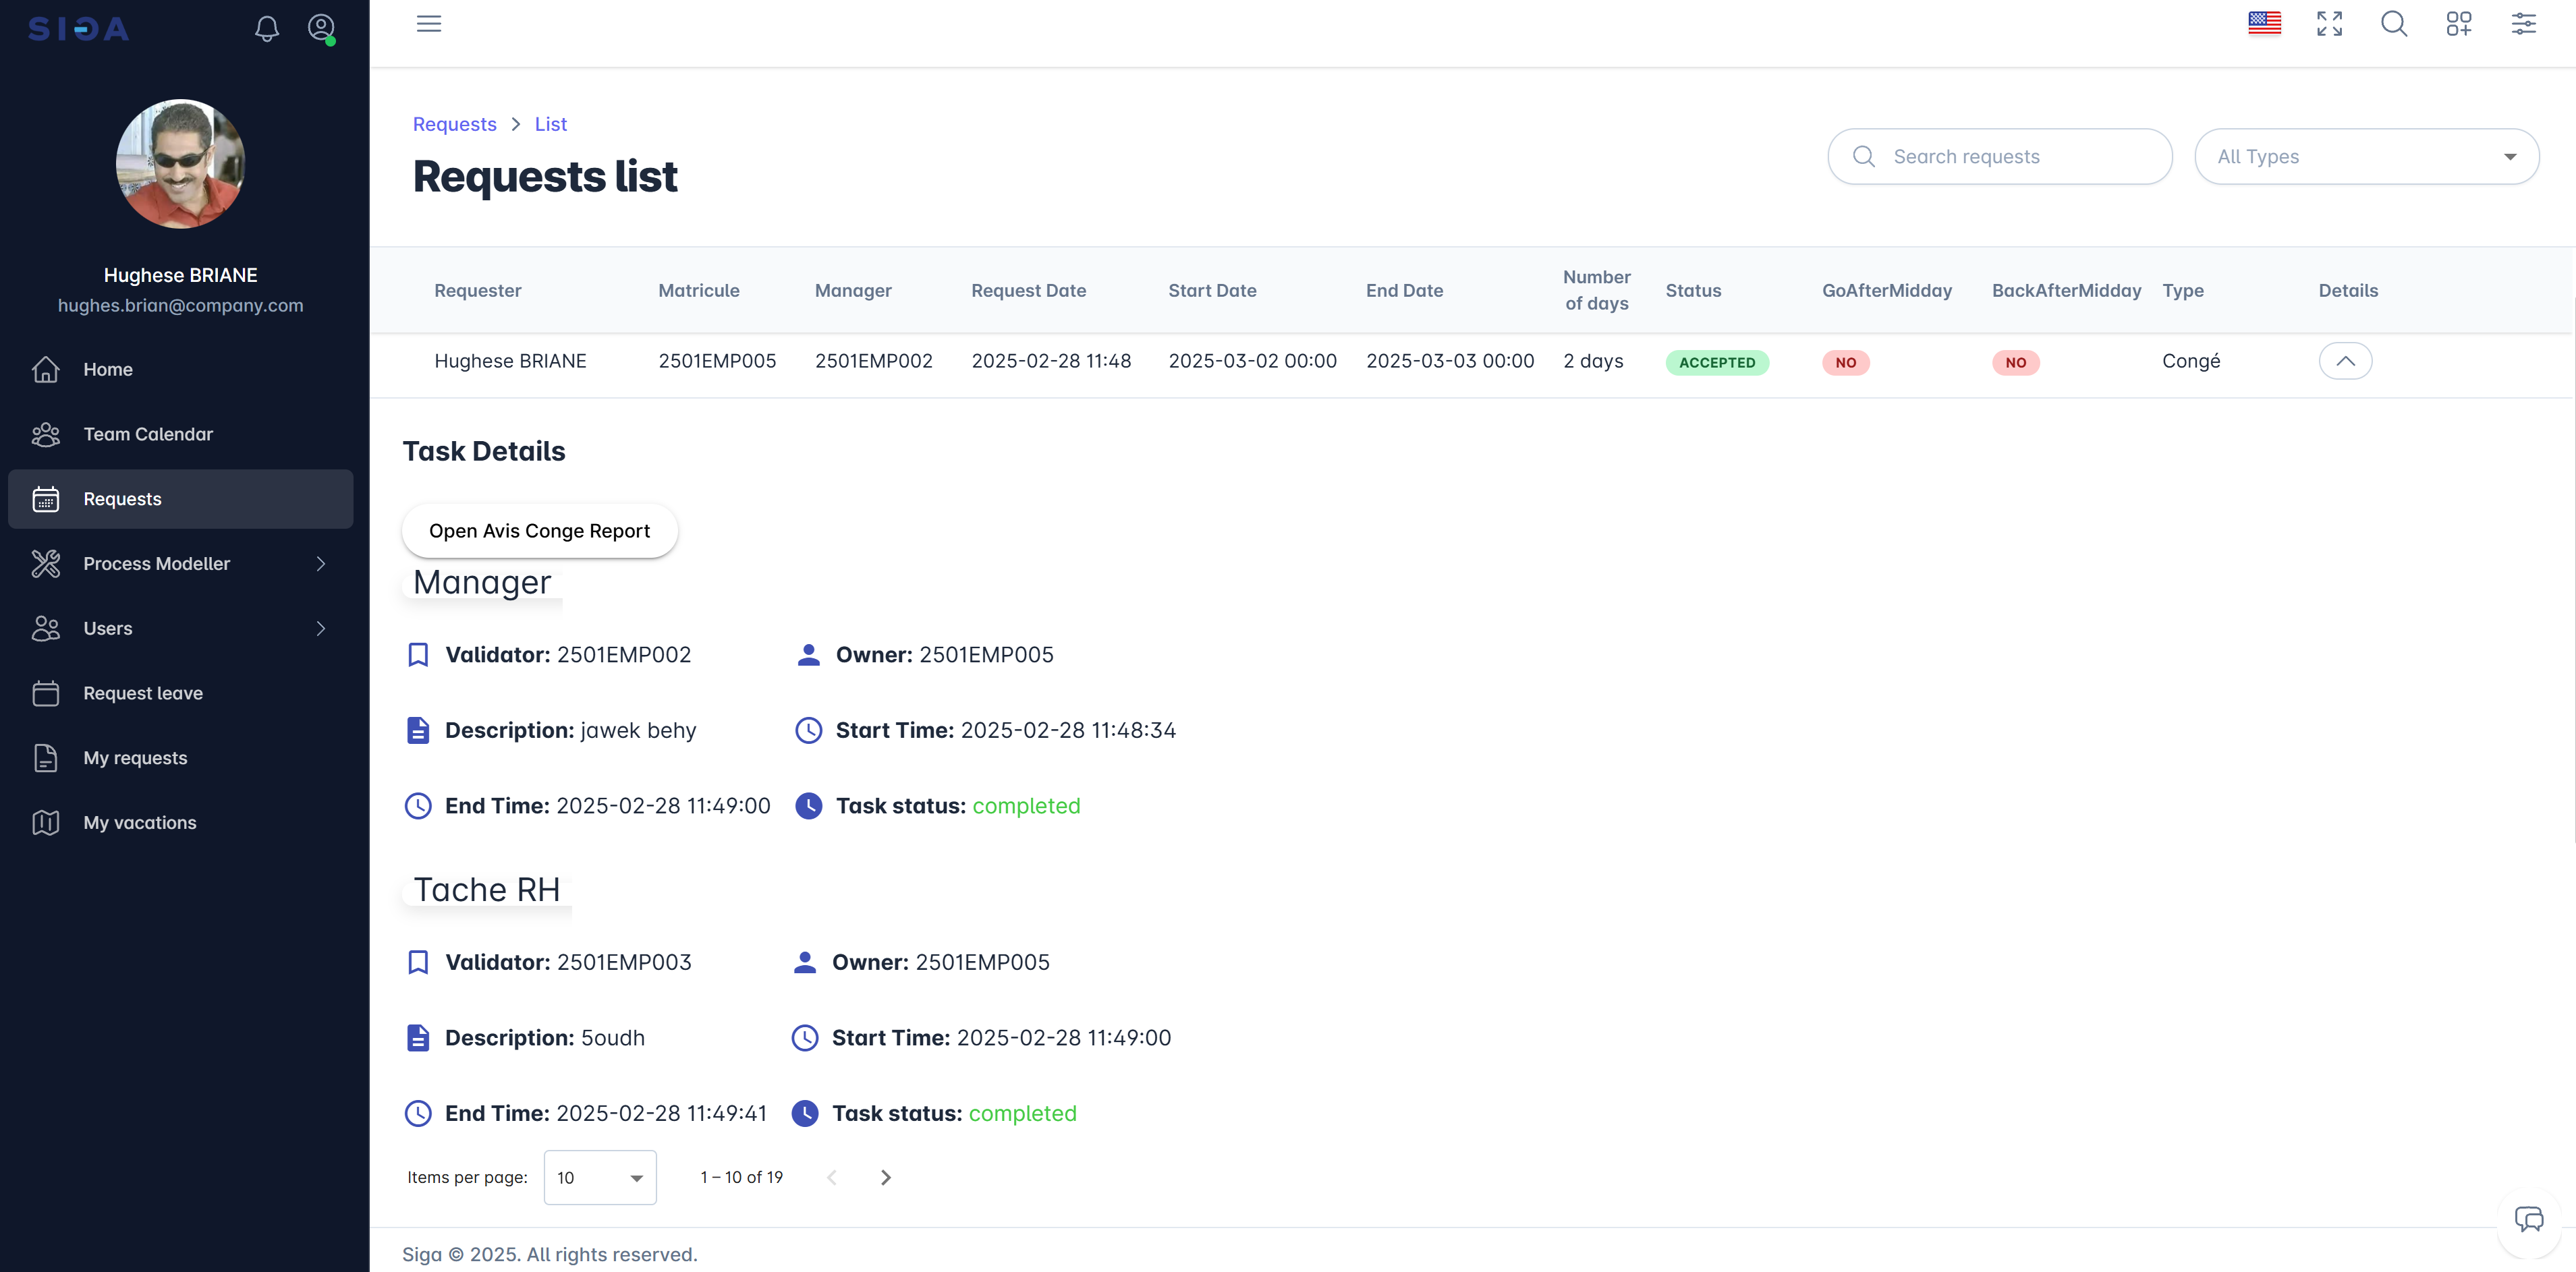
\includegraphics[width=16cm]{images/realisation/req2.png}
    \caption{Interface du cas d'utilisation «Consulter les demandes d’approbation»}
    \label{fig:demandes2}
\end{figure}    
\clearpage
\subsection{Consulter les membres de l’équipe}
La figure~\ref{fig:equipe} illustre l'annuaire interactif offrant une vue tabulaire des collaborateurs (photo, email).
\begin{figure}[h]
    \centering
    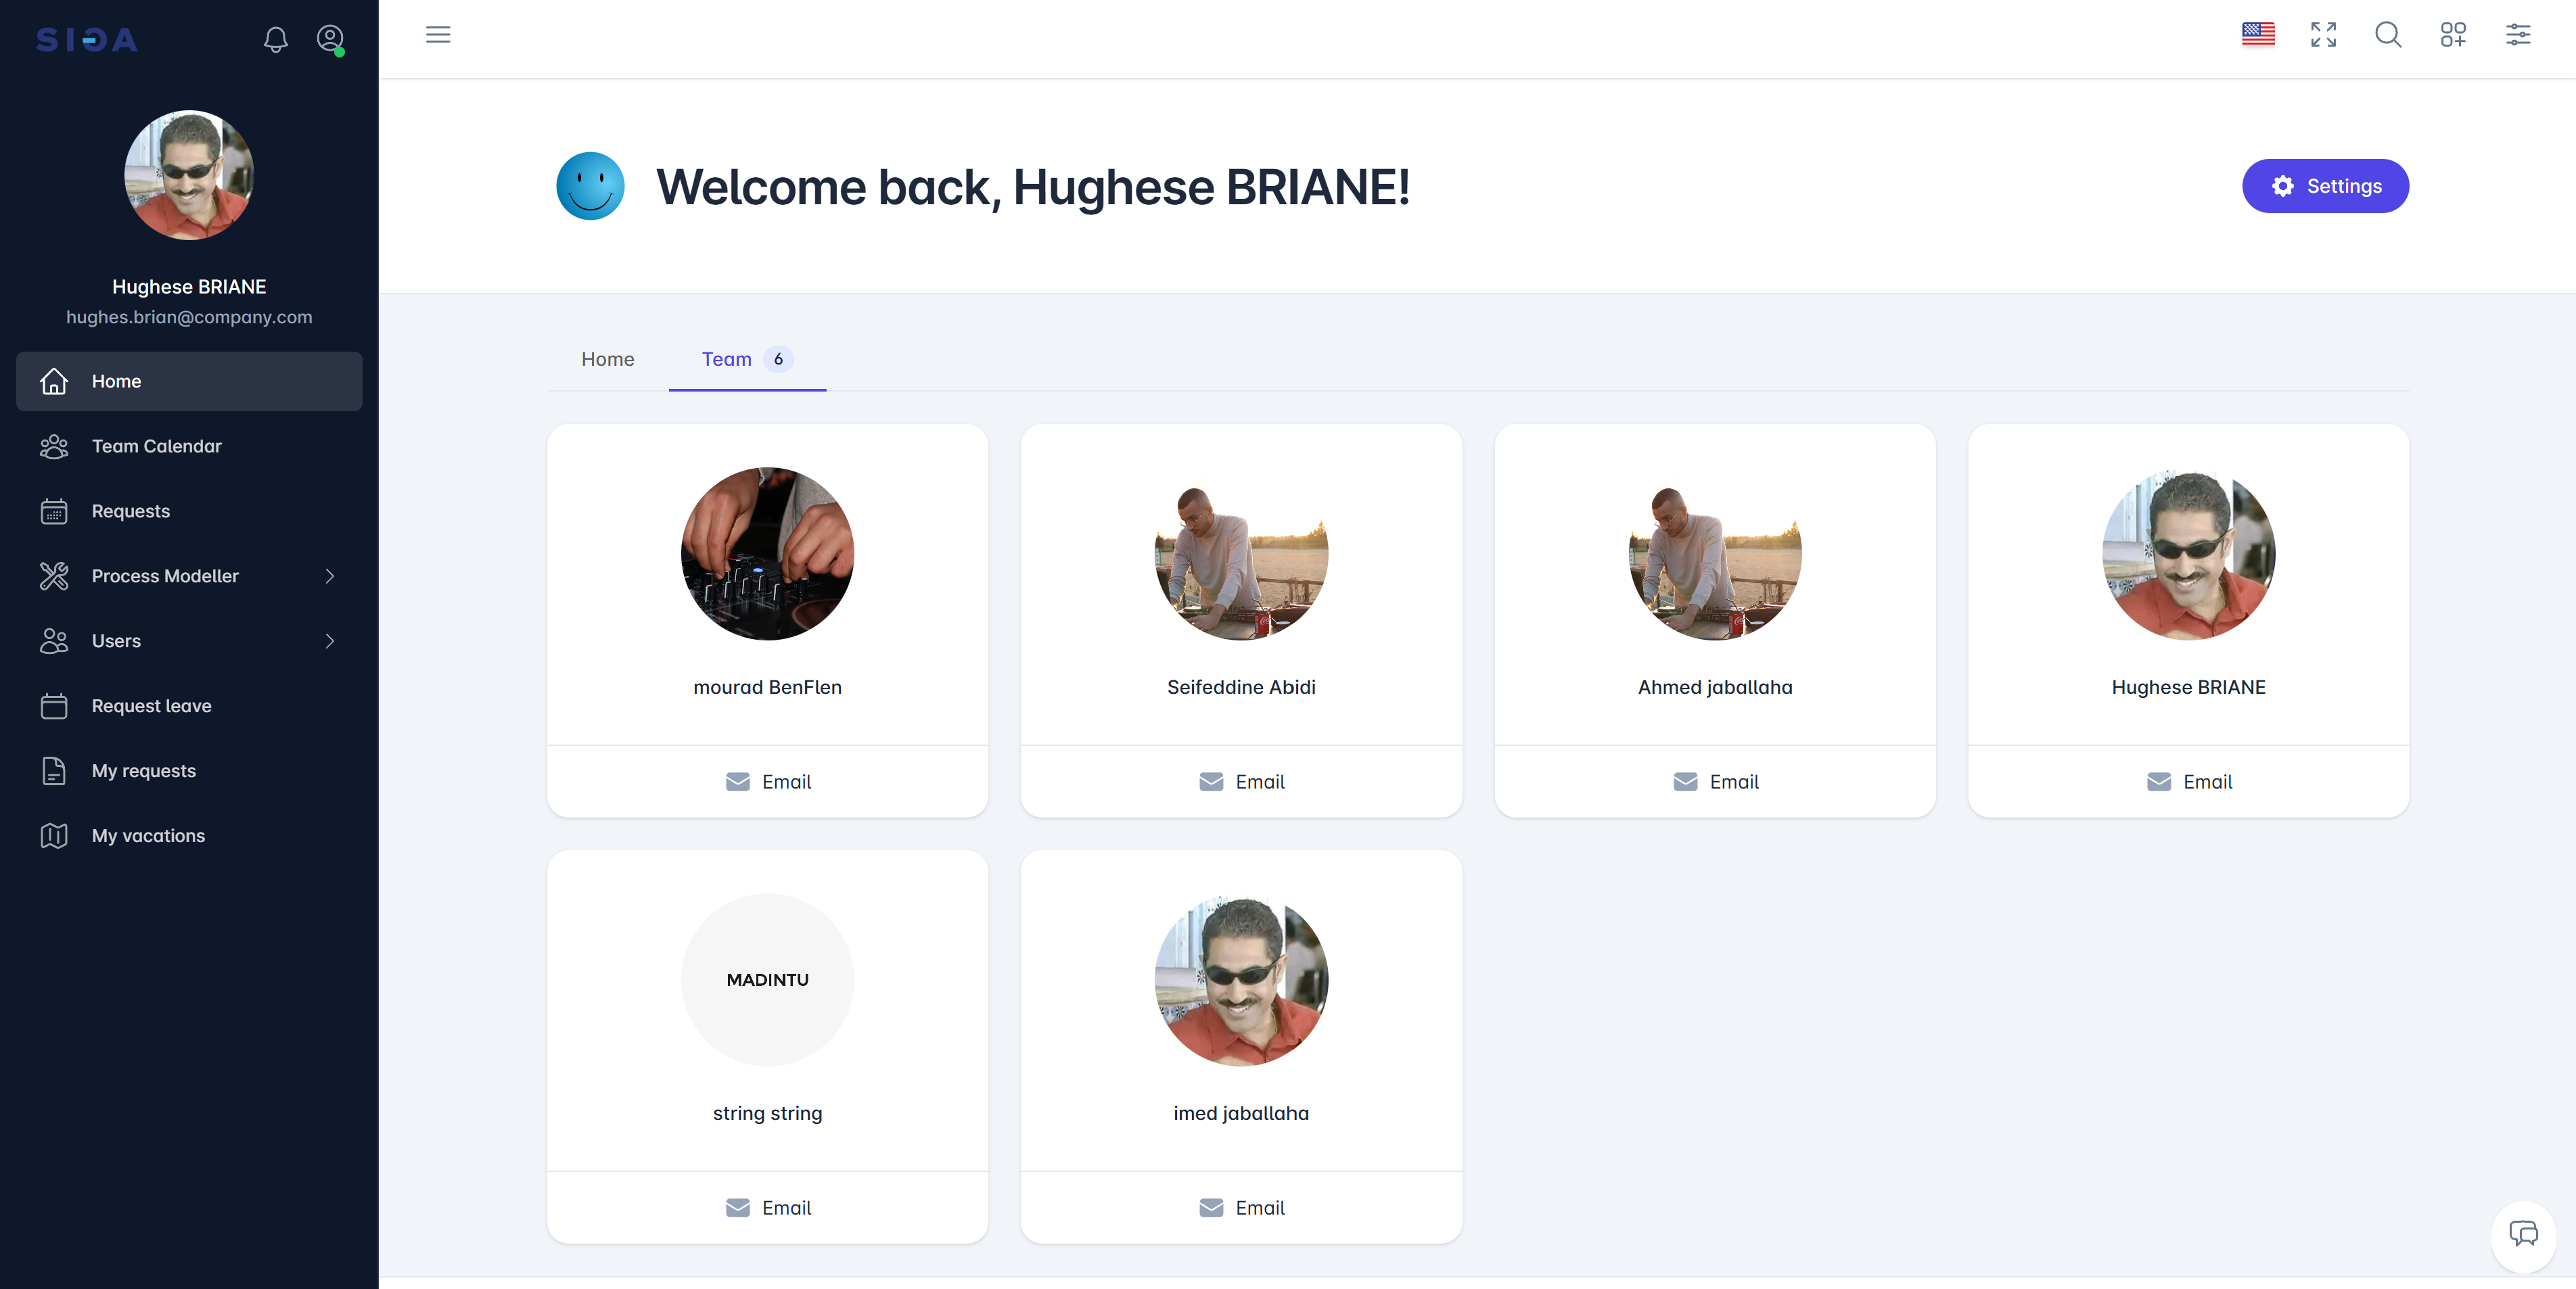
\includegraphics[width=16cm]{images/realisation/cme.png}
    \caption{Interface du cas d'utilisation «Consulter les membres de l’équipe»}
    \label{fig:equipe}
\end{figure}
\subsection{Consulter ses crédits}
Le cas d'utilisation permet aux employés de visualiser leur solde de congés et autres crédits disponibles. La figure~\ref{fig:credits} illustre l'interface dédiée.\\
\textbf{Scénario utilisateur} :
\begin{enumerate}
    \item L'utilisateur se connecte à son espace personnel
    \item Il clique sur l'onglet \textit{«Accueil»}
    \item Le système affiche :
    \begin{itemize}
        \item Le solde de congé (jours disponibles)
        \item Le solde d'autorisation (heures disponibles)
        \item L'occurence d'autorisation
    \end{itemize}
\end{enumerate}
\newpage
\begin{figure}[h]
    \centering
    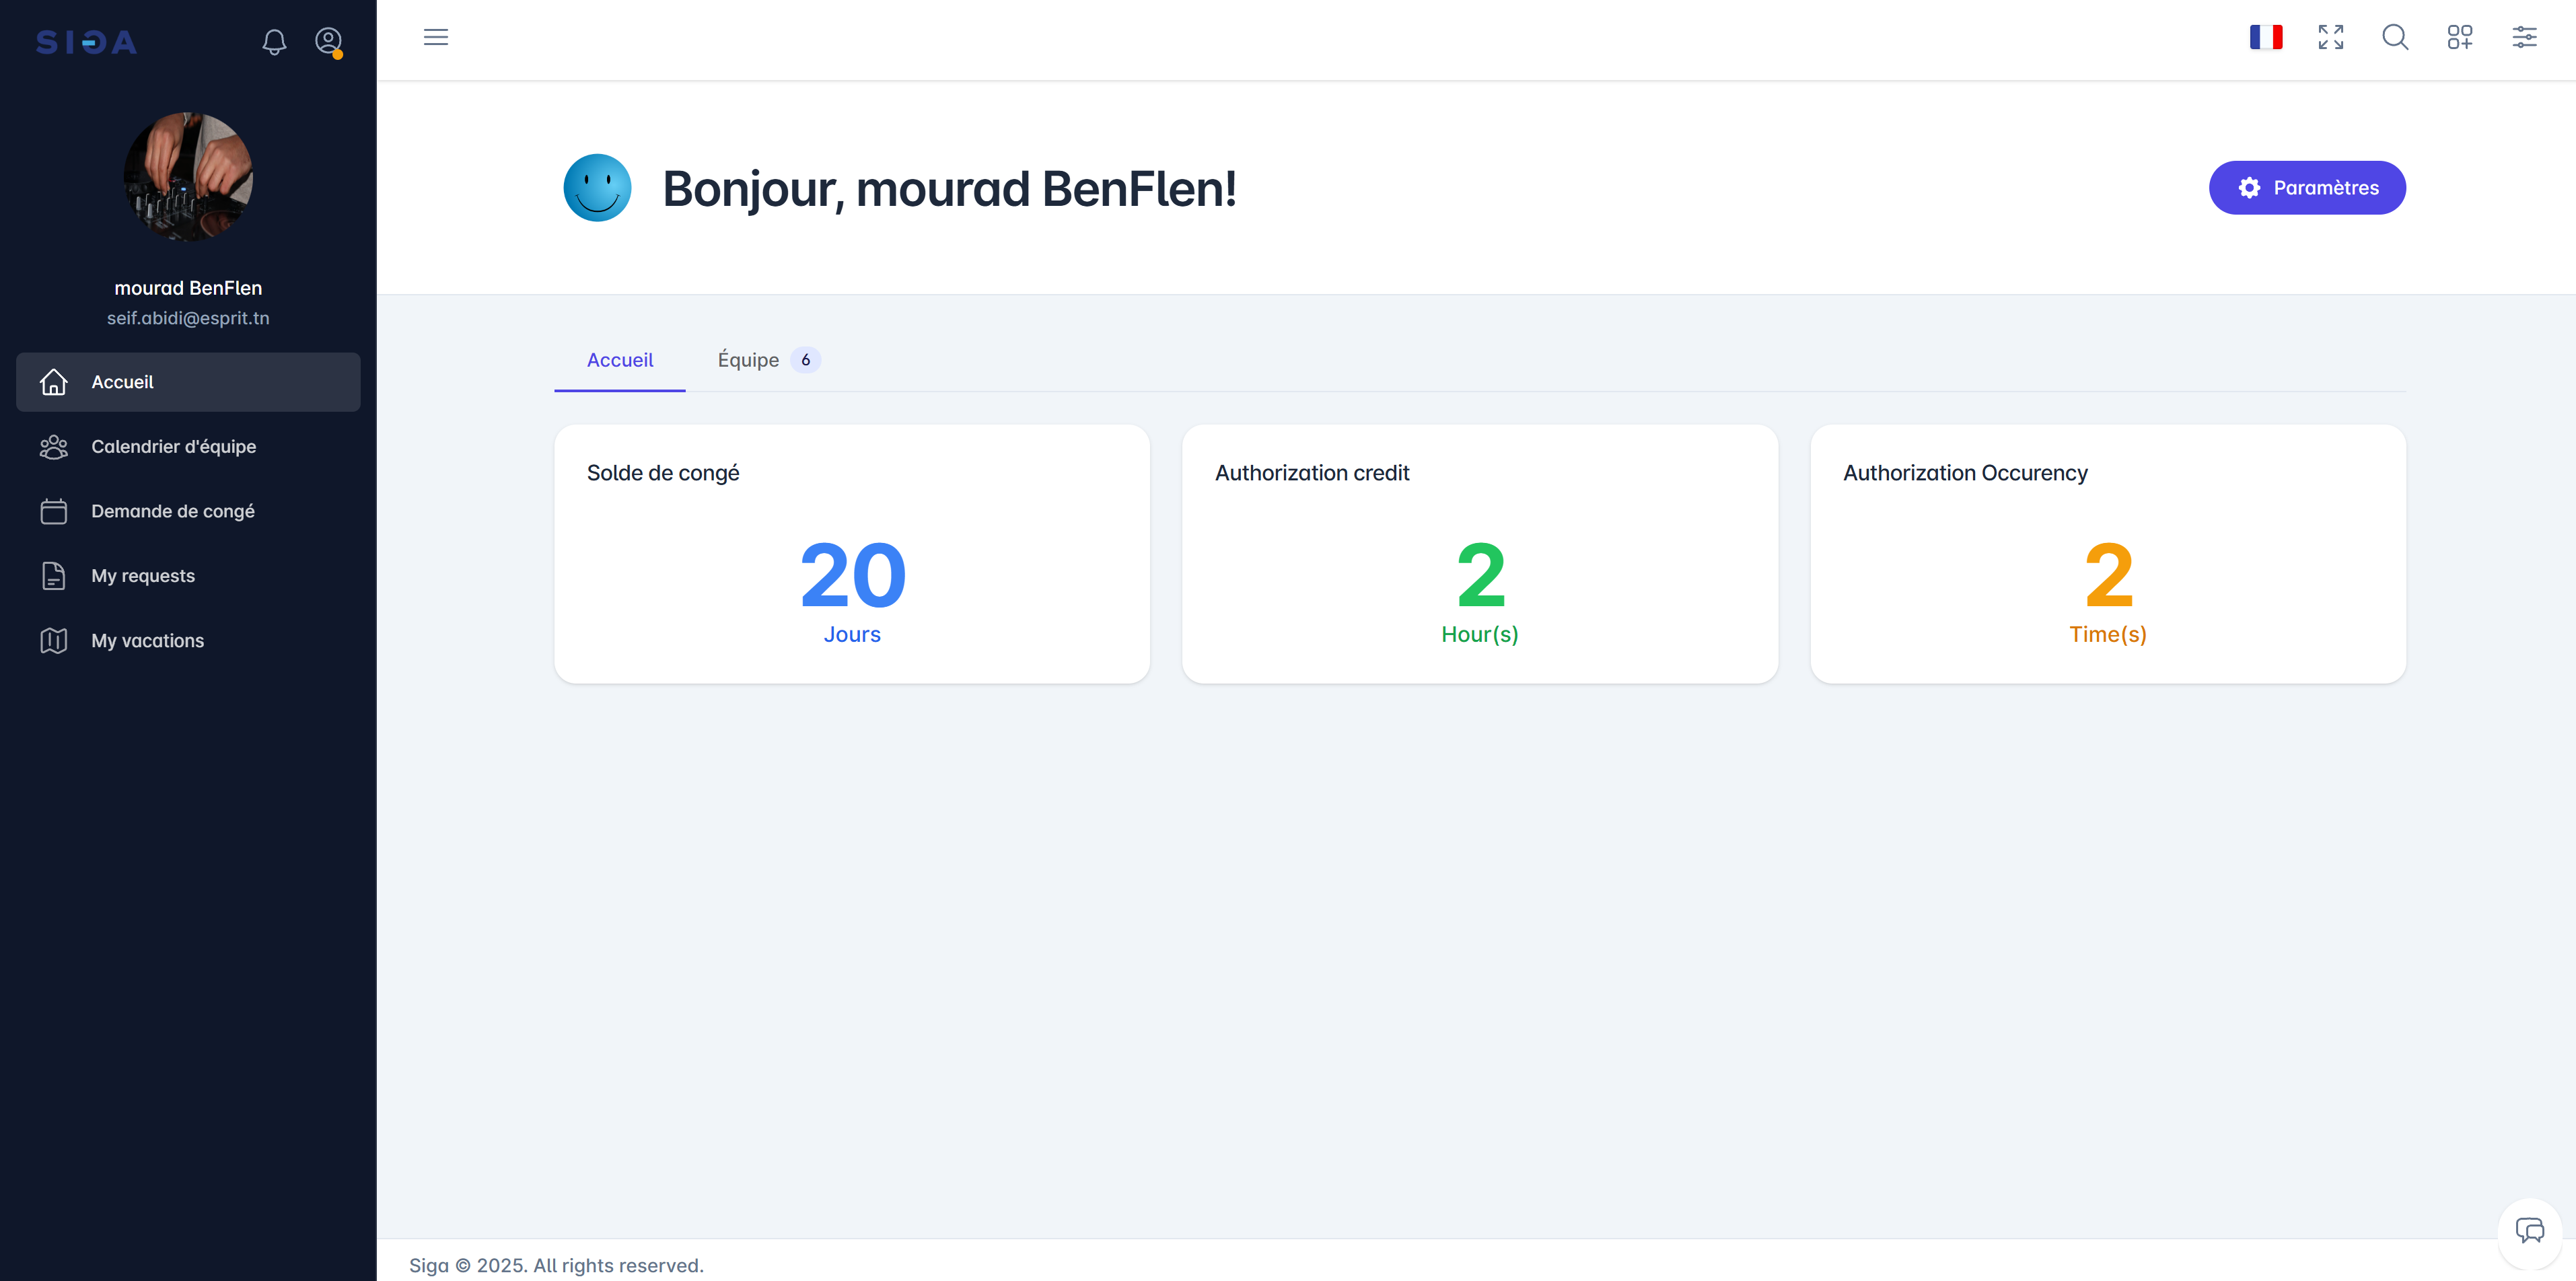
\includegraphics[width=16cm]{images/realisation/csc.png}
    \caption{Interface du cas d'utilisation «Consulter ses crédits»}
    \label{fig:credits}
\end{figure}
\section{Conclusion}
Le Sprint 3 a marqué une étape clé dans le développement de la plateforme en mettant l'accent sur le suivi et la supervision. Les fonctionnalités implémentées, telles que la réception de notifications, la consultation des processus métiers, des demandes d’approbation, des membres de l’équipe et des crédits, ont permis aux utilisateurs, managers, RH et administrateurs de mieux superviser les processus et de suivre efficacement leurs activités. 

Grâce à une conception rigoureuse, illustrée par des diagrammes de classes et de séquences, ainsi qu’une réalisation soignée avec des interfaces intuitives, ce sprint a répondu aux besoins identifiés tout en posant des bases solides pour les évolutions futures.
